\documentclass[12pt]{article}\usepackage[]{graphicx}\usepackage[]{color}
% maxwidth is the original width if it is less than linewidth
% otherwise use linewidth (to make sure the graphics do not exceed the margin)
\makeatletter
\def\maxwidth{ %
  \ifdim\Gin@nat@width>\linewidth
    \linewidth
  \else
    \Gin@nat@width
  \fi
}
\makeatother

\definecolor{fgcolor}{rgb}{0.345, 0.345, 0.345}
\newcommand{\hlnum}[1]{\textcolor[rgb]{0.686,0.059,0.569}{#1}}%
\newcommand{\hlstr}[1]{\textcolor[rgb]{0.192,0.494,0.8}{#1}}%
\newcommand{\hlcom}[1]{\textcolor[rgb]{0.678,0.584,0.686}{\textit{#1}}}%
\newcommand{\hlopt}[1]{\textcolor[rgb]{0,0,0}{#1}}%
\newcommand{\hlstd}[1]{\textcolor[rgb]{0.345,0.345,0.345}{#1}}%
\newcommand{\hlkwa}[1]{\textcolor[rgb]{0.161,0.373,0.58}{\textbf{#1}}}%
\newcommand{\hlkwb}[1]{\textcolor[rgb]{0.69,0.353,0.396}{#1}}%
\newcommand{\hlkwc}[1]{\textcolor[rgb]{0.333,0.667,0.333}{#1}}%
\newcommand{\hlkwd}[1]{\textcolor[rgb]{0.737,0.353,0.396}{\textbf{#1}}}%
\let\hlipl\hlkwb

\usepackage{framed}
\makeatletter
\newenvironment{kframe}{%
 \def\at@end@of@kframe{}%
 \ifinner\ifhmode%
  \def\at@end@of@kframe{\end{minipage}}%
  \begin{minipage}{\columnwidth}%
 \fi\fi%
 \def\FrameCommand##1{\hskip\@totalleftmargin \hskip-\fboxsep
 \colorbox{shadecolor}{##1}\hskip-\fboxsep
     % There is no \\@totalrightmargin, so:
     \hskip-\linewidth \hskip-\@totalleftmargin \hskip\columnwidth}%
 \MakeFramed {\advance\hsize-\width
   \@totalleftmargin\z@ \linewidth\hsize
   \@setminipage}}%
 {\par\unskip\endMakeFramed%
 \at@end@of@kframe}
\makeatother

\definecolor{shadecolor}{rgb}{.97, .97, .97}
\definecolor{messagecolor}{rgb}{0, 0, 0}
\definecolor{warningcolor}{rgb}{1, 0, 1}
\definecolor{errorcolor}{rgb}{1, 0, 0}
\newenvironment{knitrout}{}{} % an empty environment to be redefined in TeX

\usepackage{alltt}

\usepackage[hmargin=1in,vmargin=1in]{geometry}
\usepackage{parskip}
\usepackage{hyperref}
\hypersetup{pdfstartview=FitV,hidelinks}




\IfFileExists{upquote.sty}{\usepackage{upquote}}{}
\begin{document}


{
  \Large
  \centering
  Lab 2 assignment --- Geometric and logistic growth models \\
  Due before Monday \par
}

Answer each of the following questions by completing the provided Excel 
template and by replicating your work in R. Undergraduates should do
Exercise 1 in R, but not Exercise 2. Upload your Excel file and a
single R script to ELC before Monday. Name the files with your last
name followed by your first name. \\ 

\vspace{12pt}

{\bf Exercise 1 \\}
A study was conducted in which a population of 100 Mexican grey wolves
({\it Canis lupus baileyi}) was monitored intensively for 1 year. In
that time, 10 pups were born, and 20 of the original 100 individuals 
died. There was no immigration or emigration.  

\begin{enumerate}
  \item What are the values of $B$, $D$, $b$, $d$, $r$, and lambda
    ($\lambda$)?
  \item Assuming geometric growth, what will population size be in
    each of the subsequent 10 years? Create a graph of the results,
    including important chart elements such as axis titles. Remember,
    the geometric growth model is: $N_{t+1} = N_t + N_t r$.
\end{enumerate}

\vspace{24pt}

{
  \centering
  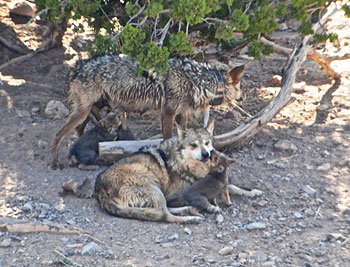
\includegraphics[width=0.7\textwidth]{figs/Coronadopack2} \\
}


\clearpage

% {\bf Exercise 2 \\}

% Abundance data on harbor seals ({\it Phoca vitulina}) in the Wadden
% Sea are provided from 1997--2009.

% \begin{enumerate}
%   \item Assuming logistic growth, find values of $r_{max}$ and $K$
%     that provide a good fit to the data. Use trial error to find these
%     values by comparing the actual number of seals to the number of
%     seals predicted by your model. You don't have to be too
%     precise, but try to get the predicted values within $\pm 2$ of the
%     actual data.
%   \item Use your model to predict how many seals will be in the
%     population in the year 2020.
%   \item Create a graph with year on the x-axis and abundance on the
%     y-axis. Show the data and the model predictions as separate
%     lines. 
% \end{enumerate}

% \vspace{24pt}

% {
%   \centering
%   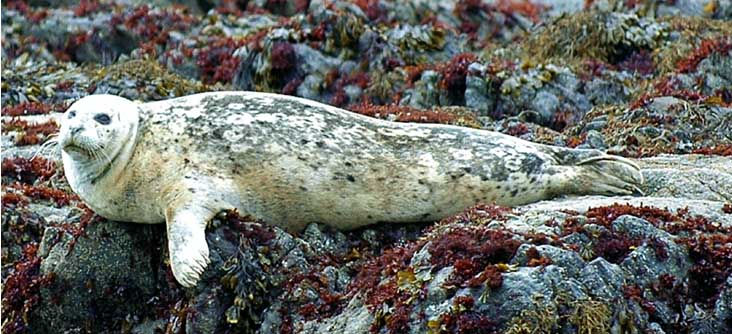
\includegraphics[width=0.8\textwidth]{figs/pacific-harbor-seal} \\
% }



% \clearpage

{\bf Exercise 2a \\}
Many people assume that the human population acts differently than
most wildlife populations and is increasing at an exponential rate, or
close to it. The UN estimated that the human population was approximately 6
billion people in 1999, and 7 billion in 2012. 

\begin{enumerate}
  \item Given this data and the (multi-step) geometric growth equation:
    $N_t = N_0(1+r)^t$, calculate $r$ for the human population over
    this 13-yr period. You will need to recall how to solve algebraic
    equations with exponents. Google it if you forgot.
  \item Use the (single-step) geometric growth equation ($N_{t+1} = N_t + N_t r$)
    and the value of $r$ that you calculated above to predict the
    human population size from 2013--2021.
  \item Graph your results.
  \item How closely does your model's prediction compare to the actual
    human population size in 2021? You can find the current population
    size here: \url{
      https://www.worldometers.info/world-population/
    }. More data about the world population can be found here: \url{
      https://ourworldindata.org/world-population-growth      
    }. Write your answer in the Excel sheet.
\end{enumerate}

\vspace{24pt}

{\bf Exercise 2b \\}
UN data on human population size from 1999 to 2012 are provided on
sheet ``Exercise 2b''.


\begin{enumerate}
  \item Calculate the population growth rate (``lambda'':
    $\lambda_t = N_{t}/N_{t-1}$) for each year starting in 2000.
  \item Using a starting values of 6 billion people in 1999, pick
    values of $r$ that make a geometric growth curve
    closely approximate the actual data. Use trial and error to find a
    good value of $r$. 
  \item The logistic growth model is: 
    $N_{t+1} = N_t + N_t r_{\rm max}(1 - N_t/K)$ where $r_{\rm max}$
    is the maximum growth rate and $K$ is the carrying capacity.
    Using a starting values of 6 billion people in 1999, pick
    values of $r_{max}$ and $K$ that make a logistic growth curve
    closely approximate the actual data. Again, use trial and error to
    find good parameter values. 
  \item Use the values you calculated above to make four graphs of:
    \begin{itemize}
      \item Actual abundance ($N$) over time
      \item Lambda ($\lambda_t$) over time
      \item Predicted geometric growth over time
      \item Predicted logistic growth over time.
    \end{itemize}
  \item Is recent human population growth more similar to geometric or
    logistic growth? Be explicit about how the observed trends of
    abundance and $\lambda_t$ indicate how the human population is
    growing. Write your answer (3--4 sentences) in the Excel sheet.
\end{enumerate}



\newpage

{\bf R tips \\}


Here's an example of a logistic growth model.
\begin{knitrout}
\definecolor{shadecolor}{rgb}{0.969, 0.969, 0.969}\color{fgcolor}\begin{kframe}
\begin{alltt}
\hlstd{rmax} \hlkwb{<-} \hlnum{0.1}              \hlcom{## max growth rate}
\hlstd{K} \hlkwb{<-} \hlnum{200}                 \hlcom{## carrying capacity}
\hlstd{years} \hlkwb{<-} \hlnum{2001}\hlopt{:}\hlnum{2050}       \hlcom{## years}
\hlstd{nYears} \hlkwb{<-} \hlkwd{length}\hlstd{(years)}
\hlstd{N1} \hlkwb{<-} \hlkwd{rep}\hlstd{(}\hlnum{NA}\hlstd{, nYears)}
\hlstd{N1[}\hlnum{1}\hlstd{]} \hlkwb{<-} \hlnum{100}             \hlcom{## abundance in first year}
\hlcom{## for loop}
\hlkwa{for}\hlstd{(t} \hlkwa{in} \hlnum{2}\hlopt{:}\hlstd{nYears) \{}
    \hlstd{N1[t]} \hlkwb{<-} \hlstd{N1[t}\hlopt{-}\hlnum{1}\hlstd{]} \hlopt{+} \hlstd{N1[t}\hlopt{-}\hlnum{1}\hlstd{]}\hlopt{*}\hlstd{rmax}\hlopt{*}\hlstd{(}\hlnum{1} \hlopt{-} \hlstd{N1[t}\hlopt{-}\hlnum{1}\hlstd{]}\hlopt{/}\hlstd{K)}
\hlstd{\}}
\hlkwd{plot}\hlstd{(years, N1,} \hlkwc{type}\hlstd{=}\hlstr{"l"}\hlstd{,} \hlkwc{xlab}\hlstd{=}\hlstr{"Year"}\hlstd{,} \hlkwc{ylab}\hlstd{=}\hlstr{"Abundance"}\hlstd{,}
     \hlkwc{main}\hlstd{=}\hlstr{"Logistic growth"}\hlstd{)}
\end{alltt}
\end{kframe}

{\centering \includegraphics[width=0.8\textwidth]{figure/logistic-1} 

}


\end{knitrout}



\end{document}

